\section{Graph\textsc{WCOJ}} \label{sec:graphwcoj}

\subsubsection{Combining \textsc{LFTJ} with \textsc{CSR}}
For our graph pattern matching specialized Leapfrog Triejoin version we choose \textsc{CSR} (see \cref{subsec:csr-background}) as
backing data structure.
This data structure is typically used for static graphs and we show that it is a great match for \textsc{LFTJ}.
In this section, we shortly describe the implementation of a \textsc{CSR} based \textit{TrieIterator}, point out the differences between
this new version and a column based \textit{TrieIterator} (as described in~\cref{ssec:seq-implementation}) and conclude with an experiment demonstrating the power of this optimization.

The implementation of a \textsc{CSR} based \textit{TrieIterator} is straightforward except for one design change: instead of using
the vertice identifier from the graph directly, we use their indices in the \textsc{CSR} representation.
This change is rather minor because it can be contained at any level by using a hash map for translation, e.g. in the
\textit{TrieIterator} itself, in the \textit{LeapfrogTriejoin} or at the end of the query by an additional mapping operation.

In the current system, the translation is performed by the \textsc{LFTJ} implementation to allow easy integration into other projects.
However, it is possible to work on the indices throughout the whole system to safe the translation costs.

We now outline how to implement each of the \textit{TrieIterator} methods, under the assumption that all vertices have outgoing edges.
Then, we drop this assumption and explain the necessary changes.
The creation of the \textsc{CSR} data structure itself is described in~\cref{subsec:spark-integration-graphWCOJ}.

We recall that a CSR uses two arrays to represent the graph edge relationship;
the \textit{AdjacencyLists} array and \textit{Indices} array.
The first one stores all ajacency lists in one direction (outgoing or incoming) as one concatenated array.
The second stores indices into the first array, e.g. the value 5 at the position 1 means that the adjacency list
for the second vertice starts at the 5th position in \textit{AdjacencyLists}.

The vertical component of the \textit{TrieIterator} consists out of the \textit{open} and \textit{up} methods.
Both of them control on which of the two \textsc{CSR} arrays the iterator is operates.
For the first level, it uses the \textit{Indices} array and on the second level the \textit{AdjacencyLists} array.

The \textit{open} method does nothing when the first level is opened.
When the second level is opened, it positions the iterator at the first element of the adjacency list.
This position is given by the index in \textit{Indices} where the first level is positioned.

Both methods use only a constant time.
This differs from the \textit{open} method of the array based \textit{TrieIterator}.
This method needs to find the number of second level elements when the second level is opened;
it does so by counting the number of occurrences of the first level key in the first column.
Additionally, both vertical component methods have more book keeping overhead for the array based implemenation.

The linear component of the \textit{TrieIterator} is made of the functions: \textit{key}, \textit{atEnd}, \textit{seek} and
\textit{next}.

The \textit{key} and \textit{atEnd} method are both only returning values computed by \textit{next} or \textit{seek}.
They do not differ for the \textsc{CSR} based and array based \textit{TrieIterator}.

The \textit{next} method of the CSR based \textit{TrieIterator} only changes at the first level.
While the array based method needs to use the \textit{seek} method to find the next higher value because
it needs to jump over all entries of the same value as the current key, the CSR based value can simply increase
the iterator position by one.

The \textit{seek(key)} method exhibits the biggest possible performance improvement on the first level.
For the array based version, we need to use a binary search to find the \textit{key}.
A CSR allows us to jump to the correct position in constant time because the \textit{key} parameter is the correct
index into the array.

To resolve the assumption of no empty outgoing adjacency lists, we adapt \textit{open}, \textit{next} and \textit{seek} to skip source
positions without outgoing edges.
This is easy to detect because then \textit{Indices\[x\] == Indices\[x + 1\]}.
We can skip these cases by simple linear search until we find a valid position.
This solution is sufficient because there are only a few vertices with no outgoing edges in real-world graphs.
Therefore, this linear search does not majorly influence the run time.

The \textit{TrieIterator} implementation based on \textsc{CSR} is much faster than the column based iterator; mainly due to the fact
that the \textit{seek} method on the first level can be implemented in $\mathcal{O}(1)$, instead of $\mathcal{O}(\log n)$.
This optimization has huge potential because these searches are the most costly operations for a column based
\textit{TrieIterator}~\cite{myria-detailed}.
Note that searches on the second level are fast, due to the fact that most graphs have a low outdegree (see
\cref{subsec:graph-analysis}).

Additionally to this advantage, \textsc{CSR} based \textit{TrieIterator} do less bookkeeping because they support only 2 levels and spent
nearly no time on processing \textit{atEnd} for the second level, while a column based \textit{TrieIterator} needs to calculate the
number of outgoing edges for each source vertice in its \textit{open} method, to allow a fast \textit{atEnd} method.

We conclude that \textsc{CSR} based \textit{TrieIterator}'s are a promising match for \textsc{LFTJ} and graph pattern matching.
The improvements of this optimization can be seen in \cref{fig:wcoj-vs-graphWCOJ}.
It demonstrates an up to 2.6 speedup over a column based \textsc{LFTJ}. % NUMBER
We also see that the optimization has a stronger impact on queries with more edges and vertices, e.g. \texttt{5-clique}.
For a more thorough evaluation refer to the experiment section \ref{sec:experiments}.

\begin{figure}
\centering
\includegraphics[width=0.5\textwidth]{wcoj-vs-graph-wcoj.png}
\caption{Barchart comparing join time of \texttt{WCOJ} and \texttt{GraphWCOJ} on multiple queries on \texttt{SNB-sf1}}
\label{fig:wcoj-vs-graphWCOJ}
\end{figure}

\subsubsection{Exploiting low average outdegrees}
% TODO study in backgrounda

In our study of real-world graphs (\cref{sec:graph-analysis}), we show that most real-world graphs have a small, average outdegree.
The outdegree over all graphs is TODO and the maximum average outdegree of a single graph
is TODO at TODO.
These results lead to the hypothesis that the intersection of multiple adjacency lists is small, e.g. below 10 in many cases.

We can exploit this fact by materializing the intersections in the \textit{LeapfrogJoins} directly
in one go; instead of, generating one value at-the-time in an iterator like fashion as described in the
original paper~\cite{leapfrog}.
% TODO rename reference to leapfrog-triejoin
This is beneficial because it makes better use of data locality; we elaborate this statement in a later
paragraph.

We structure the remainder of this section as follows.
First, we shortly reiterate the most important facts about \textit{LeapfrogJoins} for this chapter.
Second, we analysis the intersection workload in terms of input sizes and result size to confirm our hypothesis
and gain valuable insights to choose the best intersection algorithm.
Third, we explain the algorithm we chose based on the analysis.
Fourth, we point out differences to the original Leapfrog Triejoin.
Finally, we present a short experiment showing the performance gains of this optimization.

% TODO synchronize with new Leapfrog section
\textit{LeapfrogJoins} build the intersection between multiple adjacency lists.
This is done in an iterator-like fashion in their \textit{leapfrog\_next} method by repeatedly finding the upper-bound for the largest
value in the lowest iterator.
This algorithm is asymptotically optimal for the problem of n-way intersections.
However, we claim that it is (1) to complex for small intersections and (2) should generate all values at once instead of one-by-one to
improve performance on real-world adjacency lists.

To determine the best algorithms to build the n-way intersection in the \textit{LeapfrogJoins},
we run some experiments to characterize the workload.
Towards this goal, we log the size of the full intersection, the size of the smallest iterator participating
and the size of the largest intersection between the smallest iterator and any other iterator on 5-clique queries on \texttt{SNB-sf-1}.
\Cref{fig:intersection-workload} depicts these metrics as cumulative histograms.
In the next paragraphs, we point out the most important observations in each of these graphs.

% TODO why is that faster, deeper in maybe on jit code or perf

\Cref{fig:intersection-workload-smallest} shows the size distribution of the smallest iterator, as to be expected for a social network
graph, the outdegree is between 1 and 200.
We do not see the long-tail distribution typical for power-law graphs because we choose the smallest iterator out of 5 and even
though there are vertices with a much higher outdegree, the chance of encountering 5 of these in a single intersection is small.
We note that in 80\% of all cases the smallest iterator has a size lower than 80 and above that the distribution slowly increases to 100\%
% NUMBER

\Cref{fig:intersection-workload-smallest-biggest} illustrates the size distribution of intersecting the smallest iterator with any other
iterator, such that the intersection is maximal.
We choose this specific metric to motivate one of our design choices later on.
As for the smallest iterator, some of these intersections are as big as ~200 but most of them are much smaller.
However, unlike for the smallest iterator metric, 80\% of the intersections contain less than 21  elements and the frequency increases to
100\% in a steep curve.

This last observation is even stronger for the size of the total intersection (\cref{fig:intersection-workload-total}):
the size is less than 5 in 80\% of all intersections and increases similarly steep to 100\%.
The maximum is lower than 200.

These observations confirm our hypothesis that the size of the intersections is small (below 5) and do not show the same long-tail
distribution as the whole social network graph.
Hence, we can materialize them without running at risk of building big intermediary results.

Furthermore, the experiment shows that optimizing by taking iterator sizes into account is worthwhile but only for the smallest iterator
because
once we start with the smallest iterator the further intersections are small (below 21) in the vast majority of all instances.


\begin{figure}[H]
\centering
\subfloat[Smallest iterator\label{fig:intersection-workload-smallest}]{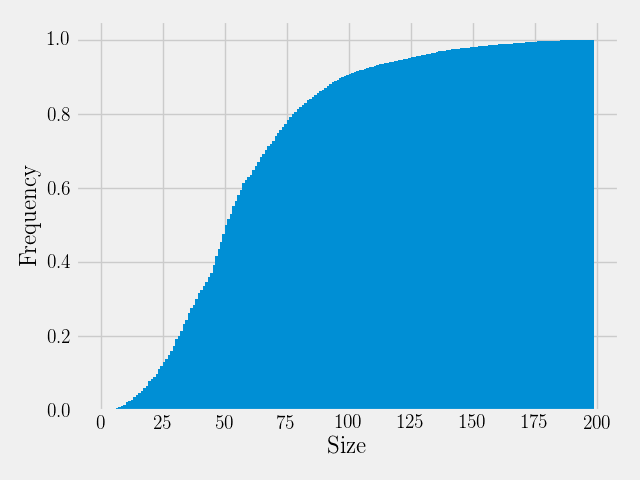
\includegraphics[width=0.3\textwidth]{intersections/smallest.png}}
\hfill
\subfloat[Largest intersection including smallest iterator\label{fig:intersection-workload-smallest-biggest}]{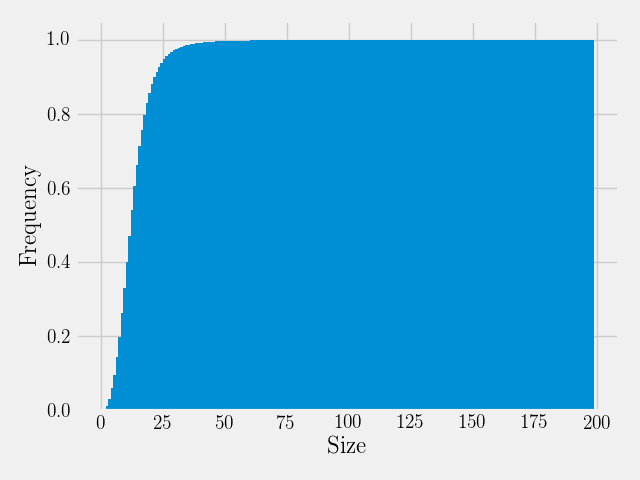
\includegraphics[width=0.3\textwidth]{intersections/smallest-biggest.png}}
\hfill
\subfloat[Total intersection\label{fig:intersection-workload-total}]{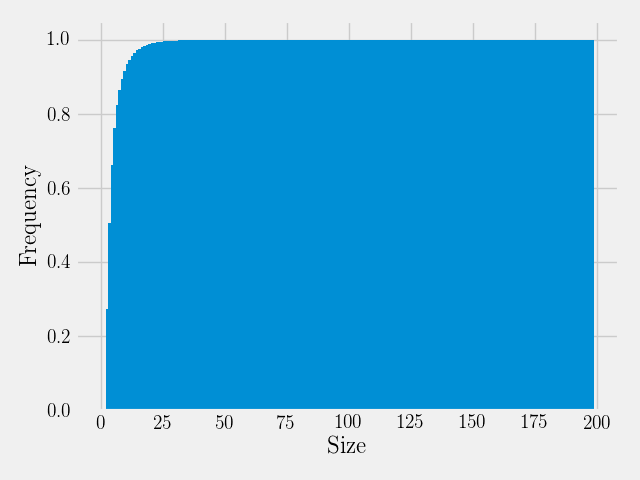
\includegraphics[width=0.3\textwidth]{intersections/total.png}}
\caption{Cumulative histograms of total intersection sizes, largest intersection with the smallest iterator and any other, and size of the
smallest iterator participating in \texttt{5-clique} on \texttt{SNB-sf-1}.}
\label{fig:intersection-workload}
\end{figure}

In the coming paragraphs, we detail how to build the n-way intersection of multiple adjacency list
such that we gain performance by better use of data-locality than original the \textit{LeapfrogJoin}.
We choose to use pairwise intersections over multi-way intersection algorithms for their simpler,
linear memory access patterns.

From our analysis, we conclude that the final intersection size is strongly dependent on the
smallest iterator and that the intersection of the smallest iterator with any other iterator is
close to the final size.
These insights translate into two design decisions.

First, we start with the smallest iterator\footnote{We take advantage of the fact that CSR allows us
to determine the size of iterators cheaply (see~\cref{ssec:csr-impl})}.
However, we do not take the sizes of any other iterators into account because the effort for
sorting the iterators by size would not pay off.

Second, we use two different tactics to build the pairwise intersections.
The first intersection between two iterators is built \textit{in-tandem},  where we seek
the upper bound of the higher value in the smaller iterator.
This algorithm guarantees to find the intersection between two iterators in the asymptotical fastest
way.
After this first intersection, the intermediary result is quite small.
Therefore, we use the simpler scheme of linearly iterating the intermediary and probing
the iterator by binary search with fall-back to linear search.

Finally, we point out a few exceptional cases and pitfalls for implementors:
\begin{itemize}
\item If all iterators of the \textit{LeapfrogJoin} are on their first level, the intersection is near |V|. In this case, we fall back
to the original
\textit{LeapfrogJoin}.
\item We use an array to materialize the intersections because Scala collections are slow.
Instead of deleting elements, we replace them with a special value.
\item Allocating a new array for every \textit{LeapfrogJoin} initialization is costly.
We estimate the size of the intersection by the size of the smallest iterator and reuse the array whenever possible. We use a sentry element to mark the end of the array.
\end{itemize}

The carefully chosen operations explained above are faster than the original \textit{LeapfrogJoin}
algorithm for two reasons.

First, the number of \textit{seek} calls to each iterator is limited by the size of the smallest iterator.
This is because the first in-tandem intersection moves the smallest iterator in each intersection
by at least one value.
All later binary intersections cause at most as many \textit{seek} calls as the size of the intermediary.

In the original algorithm, the smallest iterator is only moved every $\frac{1}{|iterators|}$ times.
Hence, the limit of \textit{seek} calls

This is due to better cache usage.
Most of the searches in the adjacency lists are linear searches;
our binary search falls back to a linear search if the remaining list is small.
Materializing the intersections means repeating linear searches for increasing elements on the same
two arrays until they are fully processed.
While the original algorithm repeats linear searches over all adjacency lists, interupted from filtering
against first level iterators and does so only until one value is found;
it then has to return to the same lists for the next elements.

Second, the \textit{Leapfrog join} generates a single value, then yields control to other parts
of the \textit{LeapfrogTriejoin} algorithm and later touches the same adjacency lists again to generate the next value.
Our approach touches the adjacency lists exactly once per \textit{LeapfrogJoin} initialization and
condenses the intersection into a much smaller array.
This array is more likely to stay cached while the other parts of the \textit{LeapfrogTriejoin} do their work.

\Cref{fig:mat-vs-nomat} shows that a materialized \textit{LeapfrogJoin} out-performance better than
the original algorithm.
As expected, the optimization is more powerful for bigger queries because they work with more
adjacency lists per \textit{LeapfrogJoin}, e.g. for a triangle each \textit{LeapfrogJoin} intersects
only two iterators while for a 5-clique each join handles 5 adjacency lists.
Anyhow, even for the triangle query, we see a small but clear improvement.

We refer the reader to our experiment section (\ref{sec:experiments}) for further experiments on
our graph specialized \textsc{wcoj} and detailed descriptions of the datasets and queries used.

\begin{figure}[H]
\centering
% TODO more queries
% TODO add amazon graph
% TODO rename dataset to materialization and no materialization or such
\includesvg[width=0.5\textwidth]{mat-graph-bar-snb-sf1}
\caption{Barchart showing \texttt{GraphWCOJ} with and without \textit{Leapfrog join} materialization
enabled for different queries on \texttt{SNB-sf1}.}
\label{fig:mat-vs-nomat}
\end{figure}